\documentclass[a4paper,12pt]{article}
%\documentclass{amsart}

\usepackage[a4paper, total={17cm, 25cm}]{geometry}
\usepackage[utf8]{inputenc}
\usepackage[english]{babel}
\usepackage{amsmath,bm,amsfonts,amssymb}
\usepackage{xcolor}
\usepackage{graphicx}
\usepackage[round]{natbib}
\usepackage{mathtools}
\usepackage[font=normalsize]{subfig}
\usepackage{float}
\usepackage{hyperref}
\usepackage{stmaryrd}%\mapsfrom
%\usepackage{cprotect}%for \verb in captions
%\usepackage{enumerate}
\usepackage{enumitem}
\hypersetup{colorlinks=true,
			linkcolor=blue,
			filecolor=blue,
			urlcolor=blue,
			citecolor=blue}
\newcommand{\mr}{\mathrm}
\newcommand{\mc}{\mathcal}
\let\SSS\S
\renewcommand{\S}{^\mr{S}}
\newcommand{\ii}{\mr{i}\,}
\newcommand{\ee}{\mr{e}}
%\newcommand{\varphit}{\psi}
\newcommand{\varphit}{\tilde\varphi}
\newcommand{\br}[3]{\left#1#2\right#3}
\let\underscore\_
\renewcommand{\_}[1]{_\mr{#1}}
\newcommand{\oo}[1]{^{(#1)}}
\newcommand{\rr}{\bm r}%{x,y}
\newcommand{\cp}{c\_p}
\let\Re\relax
\let\Im\relax
\DeclareMathOperator\Re{Re}
\DeclareMathOperator\Im{Im}
\newcommand{\w}{w}
\newcommand{\bU}{\bm U}
\newcommand{\h}{\hat}
\newcommand{\rbr}[1]{\left(#1\right)}
\newcommand{\sbr}[1]{\left[#1\right]}
\newcommand{\cbr}[1]{\left\{#1\right\}}
%\newcommand{\bU}{(\nabla\phi)_{z=\eta}}



%\newcommand{\zz}{z}
%\newcommand{\xx}{x}
%\newcommand{\yy}{y}
%\newcommand{\z}{\zeta}
%\newcommand{\x}{\xi}
%\newcommand{\y}{\sigma}
\newcommand{\z}{z}
\newcommand{\x}{x}
\newcommand{\y}{y}
\newcommand{\zz}{\zeta}
\newcommand{\xx}{\xi}
\newcommand{\yy}{\sigma}
%\newcommand{\k}{k}
\newcommand{\kk}{\kappa}

\newcommand{\zmap}{f}
%\newcommand{\zzmap}{\zmap^{-1}}
\newcommand{\zzmap}{\zmap^{\raisebox{.2ex}{$\scriptscriptstyle-1$}}}

%\newcommand{\ww}{w}
%\renewcommand{\w}{\ww^\mr{P}}
\newcommand{\ww}{\omega}
\renewcommand{\w}{w}

\newcommand{\Hz}{H}
\newcommand{\Hzz}{\tilde H}

\newcommand{\hzz}{\eta}
\newcommand{\hz}{h}
%\newcommand{\w}{\varpi}
\newcommand{\dd}[2]{\frac{\mr d #1}{\mr d #2}}

\newcommand{\Lsin}{\mc S}
\newcommand{\Lcos}{\mc C}
\newcommand{\FF}{\mc F}
\newcommand{\surf}{\eta}
\newcommand{\xS}{\x\S}
\newcommand{\tf}{\tilde \zmap}

 \newcommand{\phib}{\Phi}
 \newcommand{\wb}{W}

\DeclareMathOperator{\sech}{sech}
\DeclareMathOperator{\csch}{csch}
\begin{document}
\title{Conformal mapping in the The Higher Order Spectral method}
\author{Andreas H. Akselsen}
\date{\today}
\maketitle

%\tableofcontents

\section{Aim}
This document presents a conformal mapping approach to evaluating potential function derivatives in two dimensions at a modulated free surface.
The problem is encountered within free-surface hydrodynamics whence boundary conditions require a vertical velocity component $v=\phi_y$ evaluated at the free surface $(\x,\surf(\x))$ itself.
A standard approach for such an evaluation, e.g.\ adopted in numerical higher order spectral methods, is to related the free surface $\y=\surf$ to the horizontal line $\y=0$ through Taylor expansions.
The downside of such an approach is that the Taylor series convergence is limited \citep{west1981deep} and that it requires evaluation of a number of functional derivatives.
The number is proportional to the square of the expansion order, each requiring a pair of Fourier transformations.
\\

As will be shown, the conformal mapping approach presented here provides and explicit expression for the surface velocities for a given surface potential.
The expression does not entail any series expansions and is not subject to convergence limitations.
What's more, it requires only four Fourier transformations---the surface potential and elevation, for the surface elevation gradient and for the final vertical velocity component.

\section{Derivation}
We map the complex coordinate
$\z = \x+\ii\y$
of the physical $\z$-plane to a rectangular plane $\zz=\xx+\ii\yy$ using the conformal transformation function
\[\z\mapsfrom \zmap(\zz).\]
We wish this function to map the free surface at $\z=\x+\ii\hz(\x,t)$ to the ordinate $\zz=\xx$ of the $\zz$-plane while maintaining orthogonality to a flat bottom at $\y=-\Hz$.
For this purpose we introduce the following two transformation kernels:
\newcommand{\fun}{\mu}
\begin{subequations}
\begin{align}
\Lcos[\fun](\zz) &= \sum_{j=-\infty}^\infty \FF_j(\fun) \frac{\ee^{\ii \kk_j(\zz+\ii \Hzz)}}{\cosh(\kk_j\Hzz)} = \sum_{j=-\infty}^\infty \FF_j(\fun) \frac{2\ee^{\ii \kk_j \zz}}{\ee^{2\kk_j\Hzz}+1}\label{eq:Lcos}\\
\Lsin[\fun](\zz) &= \sum_{j=-\infty}^\infty \FF_j(\fun) \frac{-\ee^{\ii \kk_j(\zz+\ii \Hzz)}}{\sinh(\kk_j\Hzz)-\delta_j} = \sum_{j=-\infty}^\infty \FF_j(\fun) \frac{-2\ee^{\ii \kk_j \zz}}{\ee^{2\kk_j\Hzz}-1-2\delta_j}.\label{eq:Lsin}%
\end{align}%
\label{eq:L}%
\end{subequations}%
$\FF_j(\fun)$ is here the Fourier transforms $\fun=\sum_{j=-\infty}^\infty \FF_j(\fun)\ee^{\ii \kk_j \xx}$ and $\delta_j=1$ for $j=0$ and zero otherwise.
Assuming $\fun(\xx)$ is real, $\Lcos$ and $\Lsin $ have the following properties:
\begin{subequations}
\begin{align}
\Lcos[\fun](\xx) &= \fun(\xx)  -2\ii \sum_{j=1}^\infty \Im\Big[\FF_j(\fun) \ee^{\ii \kk_j\zz}\Big]\tanh(\kk_j\Hzz),\label{eq:LProps:C0}\\
\Lsin[\fun](\xx) &= \fun(\xx)  -2\ii \sum_{j=1}^\infty \Im\Big[\FF_j(\fun) \ee^{\ii \kk_j\zz}\Big]\coth(\kk_j\Hzz);\label{eq:LProps:S0}\\
\Lcos[\fun](\xx-\ii\Hzz) &= \FF_0(\fun)  +2    \sum_{j=1}^\infty \Re\Big[\FF_j(\fun) \ee^{\ii \kk_j\zz}\Big]\sech(\kk_j\Hzz),\label{eq:LProps:CH}\\
\Lsin[\fun](\xx-\ii\Hzz) &= \FF_0(\fun)  -2\ii \sum_{j=1}^\infty \Im\Big[\FF_j(\fun) \ee^{\ii \kk_j\zz}\Big]\csch(\kk_j\Hzz);\label{eq:LProps:SH}\\
\lim_{\Hzz\to\infty}\Lcos[\fun](\zz) &=\lim_{\Hzz\to\infty}\Lsin[\fun](\zz)= \FF_0(\fun) + \sum_{j=-\infty}^{-1} \FF_j(\fun) \ee^{\ii \kk_j \zz}.\label{eq:LProps:lim}
\end{align}%
\label{eq:LProps}%
\end{subequations}%
We require the property \eqref{eq:LProps:CH} at the bed for our conformal map and so we choose
\begin{equation}
\z\mapsfrom \zmap(\zz,t) = \zz+\ii\Lsin[\hzz](\zz).
\label{eq:zmap}
\end{equation}
The free surface thus obtained in the $\z$ plane is
\[\x+\ii\hz(\x,t)\mapsfrom \zmap(\xx)=\xS(\xx,t)+\ii\hzz(\xx,t).\]
Note the stretching of the $\x$ coordinate which means that 
$\hzz(\xx,t) = \hz[\xS(\xx,t),t]$ with 
\[\xS(\xx,t)=\x_0(t)+\xx+2\sum_{j=1}^\infty \Im\Big\{\FF_j[\hzz(t)] \ee^{\ii \kk_j\zz}\Big\}\coth(\kk_j\Hzz).\] 


Similar to the surface elevation, we also need to map the surface potential onto the free surface.
We introduce the complex surface potentials 
\begin{gather*}
\w(\zz,t)=\phi(\x,\y,t)+\ii\psi(\x,\y,t),
\qquad
\ww(\zz,t)=\varphi(\xx,\yy,t)+\ii\tilde\psi(\xx,\yy,t);
\\
\ww(\zz,t)=\w[\zmap(\zz,t),t]
\end{gather*}
in the two planes
%$\ww(\zz,t)$ in the $\zz$ plan, whose 
the real part is the potential function and imaginary part the stream function. 
Accordingly, 
$\Re \ww(\xx,t)=\varphi(\xx,0,t)=\varphi\S(\xx,t)=\phi[\xS(\xx,t),\hzz(\xx,t),t]$
 and $\Im \ww(\xx-\ii \Hzz,t)=\mr{const}$, and so
\begin{equation}
\ww(\zz,t) = \Lcos[\varphi\S](\zz).
\label{eq:ww}
\end{equation}


The boundary value problem reads 
\begin{align*}
h_t &=- \phi_x h_x+\phi_y,\\
%\phi_t &=- \frac12\rbr{\phi_x^2+\phi_y^2}-gh
\phi_t &=- \frac12|w_\z|^2-gh
\end{align*}
in physical space.
Re-stated in the $\zz$-plane it reads
\begin{subequations}
\begin{align}
\hzz_t\xS_\xx - \xS_t\hzz_\xx &= \phi_\y\xS_\xx-\phi_\x\hzz_\xx = \ldots = \varphi_\yy \label{eq:BC_zz:eta} \\
\varphi\S_t &= \Re(\ww_\zz f_t/ f_\zz)  - \frac12 |\ww_\zz/ f_\zz|^2  - g \hzz,\label{eq:BC_zz:phi}
\end{align}%
\label{eq:BC_zz}%
\end{subequations}%
$|\zmap_\zz|^{2}$ being the transformation Jacobian.%
 \footnote{Using the Cauchy--Riemann relations, the dynamic condition can further be written
$\varphi\S_t = |\zmap_\zz|^{-2} (\xS_t\xS_\xx + \hzz_t\hzz_\xx)\varphi_\zz - \frac12 |\zmap_\zz|^{-2} \rbr{\varphi_\xx^2-\varphi_\yy^2}  - g \hzz$ as per \citet{chalikov2005modeling}.} 
A final obstacle remains---the LHS of \eqref{eq:BC_zz:eta} should be written in terms of a single time derivative.
\citet{chalikov2005modeling} does this by introducing a modified map
\begin{equation}
\tf(\zz,t)\equiv\zmap_t/\zmap_\zz = |\zmap_\zz|^{-2}[\x_t\x_\xx + \y_t\y_\xx +\ii(\y_t\x_\xx - \x_t\y_\xx ) ]
\label{eq:tf}
\end{equation}
The kinematic condition \eqref{eq:BC_zz:eta} can now be written
\begin{equation}
\Im \tf = |\zmap_\zz|^{-2}\varphi_\yy.
\label{eq:BC_zz2:eta}%
\end{equation}%
The additional condition that $\y_t=\Im(\tf\zmap_\zz)=0$ at $\yy=-\Hzz$ leads us to the mapping
\begin{equation}
\tf(\zz,t) = \Lsin\big[|\zmap_\zz|^{-2}\varphi_\yy\big](\zz) + \tilde x_{0}(t).
\label{eq:tfMap}
\end{equation}
(The mean of $|\zmap_\zz|^{-2}\varphi_\yy$ leads to a uniform vertical shift of the domain which is of no consequence. We therefore ignore the $j=0$ component when evaluating \eqref{eq:Lsin}.)
The real uniform component $\tilde x_{0}(t)$ is chosen to avoid a gradual horizontal drift of the domain; 
by solving 
\[\int x_t\,\mr d\xx=\int\Re(\tf \zmap_\zz) \,\mr d \xx = 0\]
one finds
\begin{equation}
%\tilde x_{0}(t) = -\sum_{j=-\infty}^\infty \frac{\kk_j \Im[\FF_j(|\zmap_\zz|^{-2}\varphi_\yy)\FF_j(\eta)^*]}{\sinh^2\kk_j\Hzz + \delta_j}.
\tilde x_{0}(t) = -2\sum_{j=1}^\infty \frac{\kk_j \Im[\FF_j(|\zmap_\zz|^{-2}\varphi_\yy)\FF_j(\eta)^*]}{\sinh^2\kk_j\Hzz}.
\label{eq:tx0}
\end{equation}
The system now reads
\begin{subequations}
\begin{align}
\eta_t&= \Im(\tf \zmap_\zz), \\
%\varphi\S_t &= \Re(\ww_\zz \tf)  - \frac12|\ww_\zz/\zmap_\zz|^2  - g \hzz,
\varphi\S_t &= \Re(\tf)\varphi_\xx  - \frac12\Re \big[(\ww_\zz/\zmap_\zz)^2\big]  - g \hzz,
%\varphi\S_t &= \Re(\tf)\varphi_\xx  - \frac12 |\zmap_\zz|^{-2} (\varphi_\xx^2-\varphi_\yy^2)  - g \hzz,
\end{align}%
\label{eq:BC_zz2}%
\end{subequations}%
the former equation simply being the definition \eqref{eq:tf} and the latter being \eqref{eq:BC_zz:phi} modified with \eqref{eq:BC_zz2:eta} (which seems to improve numerical stability).
$\zmap_\zz$ and $\tf$ is of course to be evaluated at $\yy=0$.
\\


Several types of initial conditions have been tested. 
One usually successful method is to run the normal HOS scheme with nonlinearity ramping for an initial period to generate initial conditions.
A better method is to extract the initial conditions form a stationary wave solution generated with the SSGW \citep{clamond2018accurate} method;
the surface potential is easily obtained by integrating
\[\w = \int_{\Omega\S}\! \w_\z \,\mr d z\] 
along the surface line $z\in\Omega\S$. 
Both $\Omega\S$ and  $\w_\z$ are outputs of the SSGW code available online. 
The Chalikov-type HOS scheme described herein can stably maintain this wave solution for some time (stability limitations not tested yet), as shown in \autoref{fig:SSGWinit:contour} and \ref{fig:SSGWinit:eta} for a reasonably shallow wave. 


\begin{figure}[h!ptb]%
\centering
\includegraphics[width=\columnwidth]{../conformalMapping/conformalHOS/figures/imagedecayingConformalka0p2_M5_h1p00_Nw1_dt0p25T_nx512.pdf}%
\caption{Wave initiated with the SSGW solution. Steepness $k\bar H/2=0.2$, depth $H=0.1\lambda$.}%
\label{fig:SSGWinit:contour}%
\end{figure}
\begin{figure}[h!ptb]%
\centering
\includegraphics[width=\columnwidth]{../conformalMapping/conformalHOS/figures/decayingConformalka0p2_M5_h1p00_Nw1_dt0p25T_nx512.pdf}%
\caption{Wave initiated with the SSGW solution. Steepness $k\bar H/2=0.2$, depth $H=0.1\lambda$.}%
\label{fig:SSGWinit:eta}%
\end{figure}



\subsection*{Extension with a background flow field}
We can include a background flow field 
\[
%\phi(\z,t)\to\phi(\z,t)+\phib(\z,t), \qquad
\w(\z,t)\to\w(\z,t)+\wb(\z,t)\]
where $\wb(\z,t)$ is a pre-determined function representing the presence of things like wavemakers or currents.
Repeating the above derivation now yields
\begin{subequations}
\begin{align}
\Im \tf &= |\zmap_\zz|^{-2}\varphi_\yy  - \Im(\wb_\z /\zmap_\zz^*),\label{eq:BCb:kin}\\
\varphi\S_t &= -\Re(\wb_t) + \Re(\ww_\zz\tf) - \frac12\big|\ww_\zz/\zmap_\zz+\wb_\z\big|^2  - g \hzz
\intertext{or, reducing with }
\varphi\S_t &= \Re(\tf)\varphi_\xx  - \frac12\Re \big[(\ww_\zz/\zmap_\zz)^2\big]  - g \hzz
-\Re[\wb_t+\wb_\z\varphi_\xx/\zmap_\zz^*]
\end{align}%
\label{eq:BCb}%
\end{subequations}%
with $\wb_t$ and $\wb_\zz$ evaluated at $z=\zmap(\xx,t)$.
%
This expression has been validated against the previously derived model for the normal HOS method with Taylor expansion, 
\begin{align*}
\eta_t &=   - \nabla\eta\cdot\nabla\phi\S  - \nabla\eta\cdot\nabla\phib + \phib_y  + \big(1+|\nabla\eta|^2\big)\phi_y, 
\\
\phi\S_t &= -\Phi_t\big|_{z=\eta} - \frac12\big|\nabla(\phi\S +\phib)\big|^2 + \frac12\big(1+|\nabla\eta|^2\big)\phi_y^2 - g\eta,
\end{align*}
see related memo.



%$|\zmap'|^{2}$ being equivalent to the transformation Jacobian. 
%Finally, for utilization in a HOS scheme, the boundary conditions for the surface potential 
%\[
%\varphi\S(\xx,t)=\varphi[\xx+\ii\eta(\xx,t),t]
%\]
%become
%\begin{subequations}
%\begin{align}
%\eta_t &= |\zmap'|^{-2} \sbr{-   \varphi\S_\xx\eta_\xx + (1+\eta_\xx^2) \varphi_\yy},\\
%\varphi\S_t  &= |\zmap'|^{-2}\sbr{ - \frac12  \rbr{\varphi\S_\xx}^2 + \frac12 (1+\eta_\xx^2) \varphi_\yy^2 }  - g h,
%\end{align}%
%\end{subequations}%
%with  $\varphi_\yy$ evaluated at $\zz=\xx+\ii\eta$.
%$h=\Im \zmap(\xx+\ii\eta)$ is readily available. 



%Assume surface elevation $\hz(\x)$ and surface potential $\varphi\S(\x)$ known.
%
%The 
%
%
%In complex coordinates
%\[  \z = \x+\ii\y \]
%of the physical plane
%we introduce the conformal map
%\begin{equation}
%\z\mapsto\zmap(\zz) = \zz + \ii \sum_{j=-\infty}^\infty\h\surf_j \ee^{\ii k_j \zz}
%\label{eq:map}
%\end{equation}
%
%
%
%where $\h\surf_j$ are the Fourier components of the surface elevation, i.e.,\
%\[
%\surf(\x) = \sum_{j=-\infty}^\infty\h\surf_j \ee^{\ii k_j \x}.
%\]
%We use $\xx$ and $\yy$ respectively for the real and imaginary components of $\zz$; $\zz = \xx+\ii\yy$.
%Notice that 
%\begin{equation}
%\zmap(\xx) = \xx+\ii \surf(\xx),
%\label{eq:mapXi}
%\end{equation}
%i.e., $\zmap$ vartically  maps the zero-line $\zz=\xx$ onto the free surface $\z=\x+\ii\eta(\x)$.
%Conversely,
%\begin{equation}
%\zzmap(\x+\ii\surf) = \x.
%\label{eq:invMap}
%\end{equation}
%An sketch is given in \autoref{fig:map} with an example for a single harmonic in \autoref{fig:mapReg}.
%
%
%\begin{figure}[h!ptb]%
%\center
%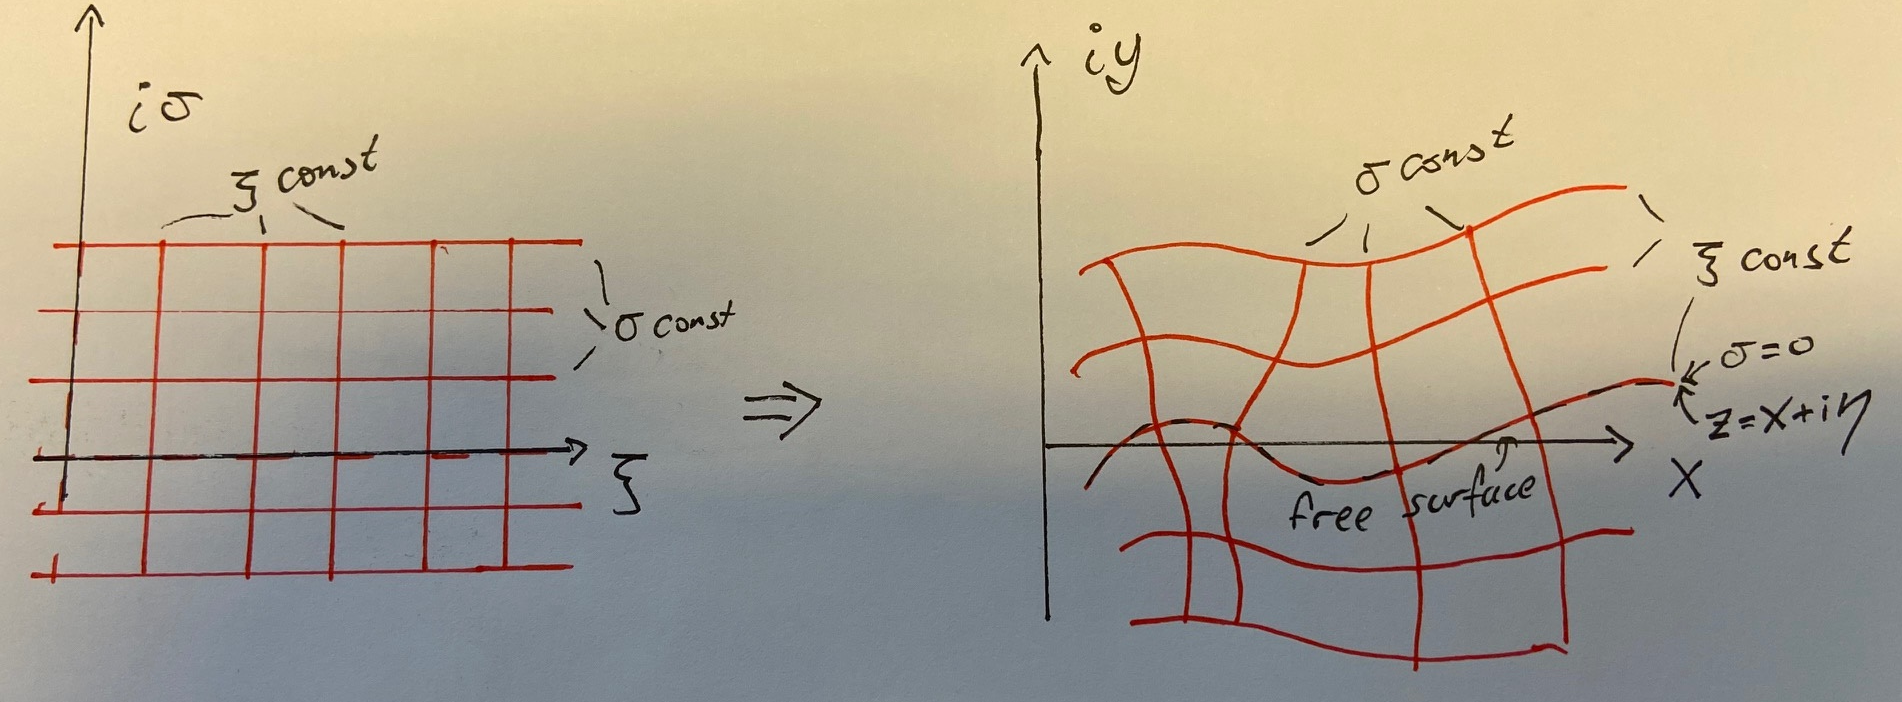
\includegraphics[width=.75\columnwidth]{./figures/map.png}%
%\caption{Conformal map, mapping line $\yy=0$ to the free surface $\y=\surf$.}%
%\label{fig:map}%
%\end{figure}
%\begin{figure}[h!ptb]%
%\centering
%\includegraphics[width=.75\columnwidth]{./conformal.pdf}%
%\caption{The map \eqref{eq:map} in the physical $\z$-plane when $\eta(\x)$ is a single harmonic of wavenumber $\pi/2$ and amplitude $0.1$.}%
%\label{fig:mapReg}%
%\end{figure}
%
%The aim of this mapping is to allow for evaluation of potential function gradients at the free surface. 
%To this endeavour, we project a complex potential filed from the rectangular $\zz$-plane onto the physical $\z$-plane,
%\begin{equation}
%%\w(\z) = \ww[\zz(\z)],
%\w(\z) = \ww[\zzmap(\z)].
%\label{eq:wProj}
%\end{equation}
%A complex potential is defined
%\[ \ww(\zz) = \varphi(\xx,\yy) + \ii \psi(\xx,\yy), \]
%$\varphi$ being the potential function and $\psi$ the stream function in the rectangular plane.
%%We have available the free surface values of the potential function $\varphi\S(x)$ and so the function matching is
%We have available the potential $\varphi\S(\x)$ at the free surface of the physical $\z$-plane, which constitutes the line $\yy=0$ in the rectangular  $\zz$-plane. 
%Accordingly, we match the functions
%\begin{equation}
%%\Re \w(x+\ii\surf) = \Re \ww(x) = \varphi\S(x).
%\varphi\S(\x) = \Re \w(\x+\ii\surf) = \Re \ww[\zzmap(\x+\ii\surf)] = \Re \ww(\x).
%\label{eq:wMatch}
%\end{equation}
%Equations \eqref{eq:invMap} and \eqref{eq:wProj} were here invoked to demonstrate the matching.
%The deep water
%%\footnote{In intermediate depth $h$, $\ww(\zz) = \sum_{j=0}^\infty a_j \frac{\sin k_j(\zz+\ii h)}{\cosh k_j h}$.}
 %complex potential is in the rectangular plane defined as a combination of positive wavenumber Fourier modes
%\begin{equation}
%\ww(\zz) = \sum_{j=0}^\infty \h\ww_j \ee^{-\ii k_j \zz}; \quad k_j\geq 0
%\label{eq:w}
%\end{equation} 
%that decay in the positive $\yy$ direction.
%Matching condition \eqref{eq:wMatch} yields
%\begin{equation}
%\h\ww_0 = \h\varphi_0\S, \quad \h\ww_j = 2\big(\h\varphi\S_j\big)^*;\; j>0, 
%\label{eq:aj}
%\end{equation}
%$\{\h\varphi\S_j\}$ being the Fourier components of $\varphi\S(x)$ and asterisk denoting the complex conjugate.
%
%We now have the ingredients necessary to compute the velocities $U=u+\ii v$ at the free surface. 
%The chain rule yields
%\begin{equation*}
%%U^* = \dd{\w}{\z}\bigg|_{0} = \dd{}{\z}\ww[\zz(\z)]\bigg|_0 = \dd\ww\zz\dd\zz\z\bigg|_0 = \bigg(\dd\ww\zz\bigg|_0\bigg)\bigg(\dd\z\zz\bigg|_0\bigg)^{-1},
%U_0^* = \dd{\w}{\z}\bigg|_{0} = \dd{}{\z}\ww[\zzmap(\z)]\bigg|_0 = \ww'/\zmap' \big|_0,
%%\label{eq:U_derive}
%\end{equation*}
%zero denoting evaluation at surface $\z=\x+\ii\surf$, $\zz=\xx$.
%Inserting \eqref{eq:map} and \eqref{eq:w}, the full expression becomes
%\begin{equation}
%U^*(\x+\ii\surf) = \frac{1}{\ii- \surf_{\x}}\sum_{j=0}^\infty  k_j \h\ww_j \ee^{-\ii k_j \x},
%\label{eq:U}
%\end{equation}
%with, of course, $\surf_\x=\sum_{j=-\infty}^\infty\ii k_j\h\surf_j\ee^{\ii k_j \x}$.
%Expression \eqref{eq:aj} and \eqref{eq:U} is all that is needed to compute the vertical velocity at the surface in deep water. Written in terms of efficient FFT and iFFT algorithms:
%\begin{equation}
%U_j^* = \frac{-2\ii}{N} \frac{  \mr{FFT}\{k_j [\mr{FFT}(\varphi_j\S)]^* \delta_{j}^+\}}{ 1-\mr{iFFT}[k_j \mr{FFT}(\eta_j)]}
%\end{equation}
%with $N$ being the number of points/modes and $\delta_{j}^+=1$ for $k_j>0$ and zero otherwise.
%\\
%
%We remark on the unexpected explicitness of this approach. 
%Conformal mapping strategies often require inverse mapping $\zzmap$ which cannot be preformed explicitly. 
%A key feature of the problem at hand is however that we only require potential function \textit{derivatives} along a prescribed path.
%
%
%
%
%
%
%\section{The conformal mapping technique in finite water depth}
%\label{sec:finiteDepth}
%Unsurprisingly, the conformal map suggested in equation \eqref{eq:map} turns out not to be original, with similar mappings fond in e.g.~\citet{chalikov2005modeling}, although its usefulness in deep-water application in the context described above appears to be unremarked.
%The deep water assumption may at first glance may look like a minor simplification, but it is in fact essential for the explicitness and simplicity of the above scheme. 
%Let's look at the problems faced by a finite depth.
%\\
%
%The conformal map, equivalent to \eqref{eq:map}, with a finite water depth $H$ is
%\begin{equation}
%z\mapsto \zmap(\zz) = \zz - \ii \sum_{j=-\infty}^\infty \h\eta_j \frac{\ee^{\ii \kk_j(\zz+\ii H)}}{\sinh \kk_jH}.
%\label{eq:map_H}
%\end{equation}
%This map does \textit{not} have the property \eqref{eq:mapXi} but rather
%\begin{equation}
%\Im \zmap(\xx) = \surf(\xx).
%\label{eq:ImMapXi}
%\end{equation}
%The difference is that $\zmap(\xx)$ comes with a stretching of the $x$-dimension where
%\begin{equation}
%\Re \zmap(\xx) \equiv x\S(\xx) = \xx -\ii  \sum_{j=-\infty}^\infty \h\eta_j \frac{\ee^{\ii \kk_j\xx}}{\tanh \kk_j H}
%\label{eq:mapXi2}
%\end{equation}
%(the latter term also being real).
%This means that $\surf(\xx)$ in \eqref{eq:ImMapXi}, the surface boundary in the $\zz$-plane, is no functionally equivalent to the the surface $h(\x)$ in the physical plane, but rather
%$\eta(\xx)=h[x\S(\xx)]$, and it is the Fourier components of $\eta(\xx)$, not of $h(\x)$, that are required in \eqref{eq:map_H}. 
%Likewise, $\kk_j$ are the wave numbers in the $\zz$-plane, as opposed to the wavenumbers $k_j$ in the $\z$-plane.
%In other words, the mapping \eqref{eq:map_H} is highly implicit in both directions.
%It is easily plotted reversely---given a function $\eta$ in the $\zz$-plane we can compute the map \eqref{eq:map_H} and see what physical surface $h(x)$ this corresponds to.
%An example is shown in \autoref{fig:map_H} for a sinusoidal $\eta(\xx)$. Note that the surface $h(x)$ in the physical plane is not sinusoidal.
%The mapping, being impractical viewed from the $\z$-plane, can still adopt for wave simulation by reformulating the boundary problem into the $\zz$-plane and performing the time integration in Fourier-space, as done by \citet{chalikov2005modeling}.
%
%
%We remark that similar to earlier we have $\zzmap[x\S(\xx)+\ii\eta(\xx)]=\xx$, etc.
%The complex potential of finite depth is in the $\zz$-plane is
%\begin{equation}
%%\ww(\zz) = \sum_{j=0}^\infty\h\ww_j \frac{\sin k_j(\zz+\ii H)}{\cosh k_j H}; \quad \h\ww_j\in\mathbb R,\; k_j\geq 0.
%\ww(\zz) = \sum_{j=-\infty}^\infty\h\ww_j \frac{\ee^{\ii \kk_j(\zz+\ii H)}}{\cosh \kk_j H}; \quad \h\ww_{-j}=\h\ww_{j}^*.
%\label{eq:wH}
%\end{equation}
%The stretching $x\S(\xx)$ further affects the mapping of $\varphi\S(\x)$ into the coefficients $\{\h\ww_j\}$.
%
%\begin{figure}[h!ptb]%
%\centering
%\includegraphics[width=.75\columnwidth]{./conformalH.pdf}%
%\caption{The map \eqref{eq:map_H} in the physical $\z$-plane when $\eta(\xx)$ is a single harmonic of wavenumber $\pi$ and amplitude $0.075$. $H=0.75$.}%
%\label{fig:map_H}%
%\end{figure}




\bibliographystyle{plainnat} % abbrvnat,plainnat,unsrtnat
\bibliography{bib,sintef_bib} %You need a file 'literature.bib' for this.


\end{document}
